\section{Background}\label{background}
This section formalizes the iterative data cleaning and training process and highlights an example application.

\subsection{Use Case: Dollars for Docs}\label{s:usecase}
ProPublica collected a dataset of corporate donations to doctors to analyze conflicts of interest~\cite{dollarsfordocsa}. 
They reported that some doctors received over \$500,000 in travel, meals, and consultation expenses.
In order to make such strong claims about the doctors, ProPublica laboriously curated and cleaned a dataset from the Centers for Medicare and Medicaid Services that listed nearly 250,000 research donations, and aggregated these donations by physician, drug, and pharmaceutical company.
We collected the raw unaggregated data and explored whether suspect donations could be predicted with a model.
This problem is typical of analysis scenarios based on observational data seen in finance, insurance, medicine, and investigative journalism.
The dataset has the following schema:
\begin{lstlisting}[mathescape,basicstyle={\small}]
Contribution(pi_specialty$\textrm{,}$ drug_name$\textrm{,}$ device_name$\textrm{,}$
$~~~~~~~~~~~~~~~~~~~~~~~~~~~~~~~$corporation$\textrm{,}$ amount$\textrm{,}$ dispute$\textrm{,}$ status)
\end{lstlisting}

\noindent\texttt{pi\_specialty} is a textual attribute describing the specialty of the doctor receiving the donation.

\noindent\texttt{drug\_name} is the branded name of the drug in the research study (null if not a drug).

\noindent\texttt{device\_name} is the branded name of the device in the study (null if not a device).

\noindent\texttt{corporation} is the name of the pharmaceutical providing the donation.

\noindent\texttt{amount} is a numerical attribute representing the donation amount.

\noindent\texttt{dispute} is a Boolean attribute describing whether the research was disputed.

\noindent\texttt{status} is a string label describing whether the  donation was allowed under the declared research protocol. The goal is to predict disallowed  donation. 

\vspace{0.5em}

However, this dataset is very dirty, and the systematic nature of the data corruption can result in an inaccurate model.
On the ProPublica website \cite{dollarsfordocs}, they list numerous types of data problems that had to be cleaned before publishing the data (see Technical Report~\cite{activecleanarxiv}).
For example, the most significant donations were made by large companies whose names were also more often inconsistently represented in the data, e.g., Pfizer Inc., Pfizer Incorporated, Pfizer.
The data cleaning problem is to resolve this common inconsistency to a canonical name.
Duplicate representations could artificially reduce the correlation between these entities and suspected contributions.
There were nearly 40,000 of the 250,000 records that had either naming inconsistencies or other inconsistencies in labeling the allowed or disallowed \texttt{status}.
Without data cleaning, the detection rate using a Support Vector Machine was 66\%.
Applying the data cleaning to the entire dataset improved this rate to 97\% in the clean data (Section \ref{exp:dfd}).

\begin{figure}[t]
\centering
 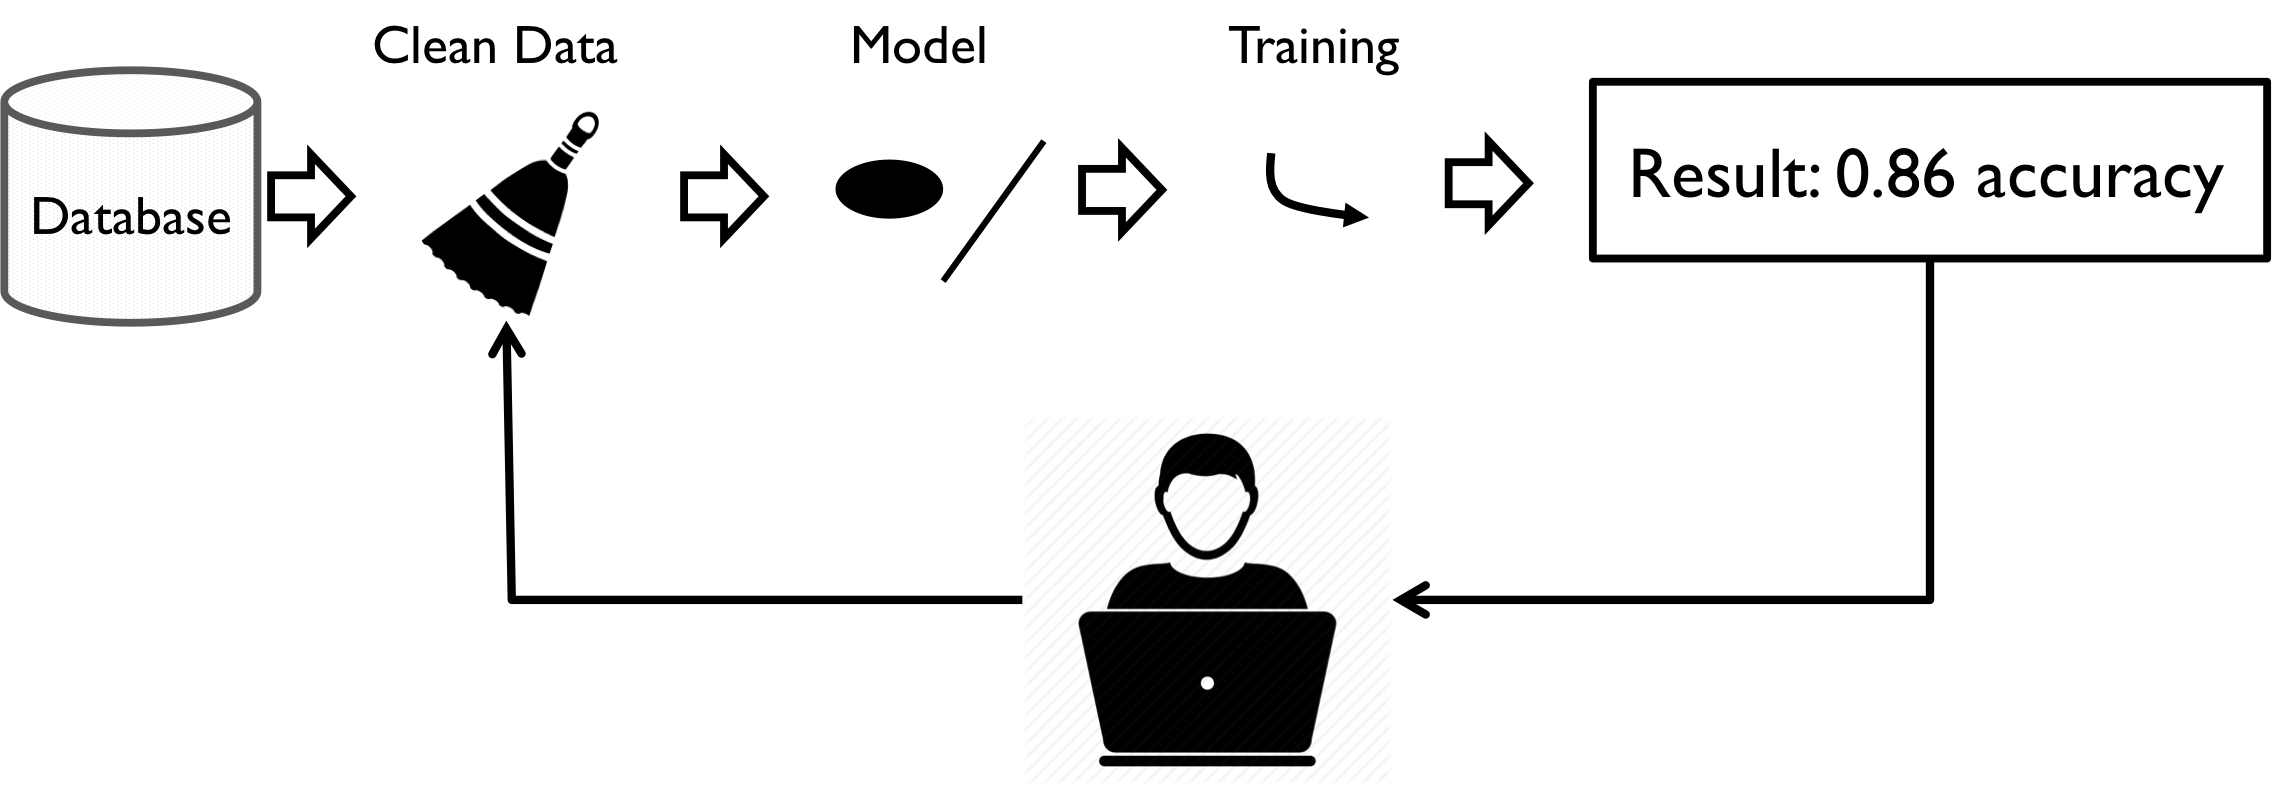
\includegraphics[width=\columnwidth]{figs/workflow.png}
 \caption{Analysts often clean data interactively with data analytics; iteratively cleaning some data and re-training on a partially clean dataset to evaluate whether the cleaning was effective. It is common to use the preliminary analysis on dirty data as a guide to help identify potential errors and design repairs. \label{cartoon}}
\vspace{-2em}
\end{figure}

\subsection{Iteration in Model Construction}
Let us consider an analyst designing an SVM classification model on the Dollars For Docs dataset.
When she develops her model on the dirty data, she will find that the detection rate (true positives predicted) is quite low 66\%.
To investigate why, she might examine those records that are labled as flagged but not predicted by the classifier.
She will then discover that there are numerous examples where two records are nearly identical but one is predicted correctly and one is incorrect, and their only difference is the \texttt{corporation} attribute: Pfizer and Pfizer Incorporated.
She will merge all records those two similar attributes, re-train the model, and repeat this process (Figure \ref{cartoon}).
There are two key challenges: correctness and efficiency.

\vspace{0.5em}
\noindent \textbf{Correctness: } Let us revist Figure \ref{update-arch1} from the introduction. 
The straight-forward application of data cleaning is to repair the corruption in-place, and re-train the model after each repair.
The problem is that aggregates over mixtures of different populations of data can result in spurious relationships due to the well-known phenomenon called Simpson's paradox \cite{simpson1951interpretation}.
Simpson's paradox is by no means a corner case, and it has affected the validity of a number of high-profile studies~\cite{pearl2003causality}.
Thus, training models on a mixture of dirty and clean data can lead to unreliable results, where artificial trends introduced by the mixture can be confused for the effects of data cleaning.

\vspace{0.5em}
\noindent \textbf{Efficiency: } An alternative is to avoid the dirty data altogether instead of mixing the two populations, and only train the model on the cleaned data.
This approach is similar to SampleClean \cite{wang1999sample}, which was proposed to approximate the results of aggregate queries by applying them to a clean sample of data.
However, high-dimensional models are highly sensitive to sample size.
Figure \ref{update-arch1}c illustrates that, even in two dimensions, models trained from small samples can be as incorrect as the mixing solution described before.
We call this the efficiency problem since while this approach is technically correct, it may converge very slowly.
One of the most popular prioritization techniques is Active Learning, which has been widely applied in the context of data cleaning~\cite{DBLP:journals/pvldb/YakoutENOI11,gokhale2014corleone}.
Active Learning considers the problem of selecting the most informative unlabeled examples to label in partially labeled static data.
Active Learning iteratively queries new examples to label and integrates those examples into the model.
In contrast, we require a broader problem of accounting for modifications to both features and labels in existing examples.
Thus, the data actually changes iteration to iteration.
Furthermore, the existing dirty attribute values may give us valuable information about the model. 
%This would be like Active Learning, where instead of unlabled data, there are inaccurate prior estimates for the labels.
%\sys reduces to a form of Expected Gradient Length Active Learning when there is no structure in the dirty data to exploit (such as completely missing attribute values).




